\section{Технический проект}
\subsection{Общая характеристика организации решения задачи}
Вы должны спроектировать и разработать алгоритмическую библиотеку. библиотека реализована на Python.

\subsection{Описание используемых библеотек и языков программирования}
Проект реализован с использованием языка Python.


\subsection{Технические детали проекта}
\subsubsection{Интерфейс редактора}
Интерфейс библиотеки алгоритмов состоит из панели поиска для фильтрации результатов по названию алгоритма, левой боковой панели с раскрывающимся списком всех алгоритмов, текстового поля с правой стороны для отображения содержимого выбранного алгоритма и кнопки для переключения режимов..

\subsection{Структура проекта}

\subsubsection{Диаграмма классов}
На рисунке 3.1 показана диаграмма классов для моего проекта Библиотека алгоритмики. Эта диаграмма иллюстрирует взаимодействие между различными классами.


\begin{figure}[H]
	\centering
	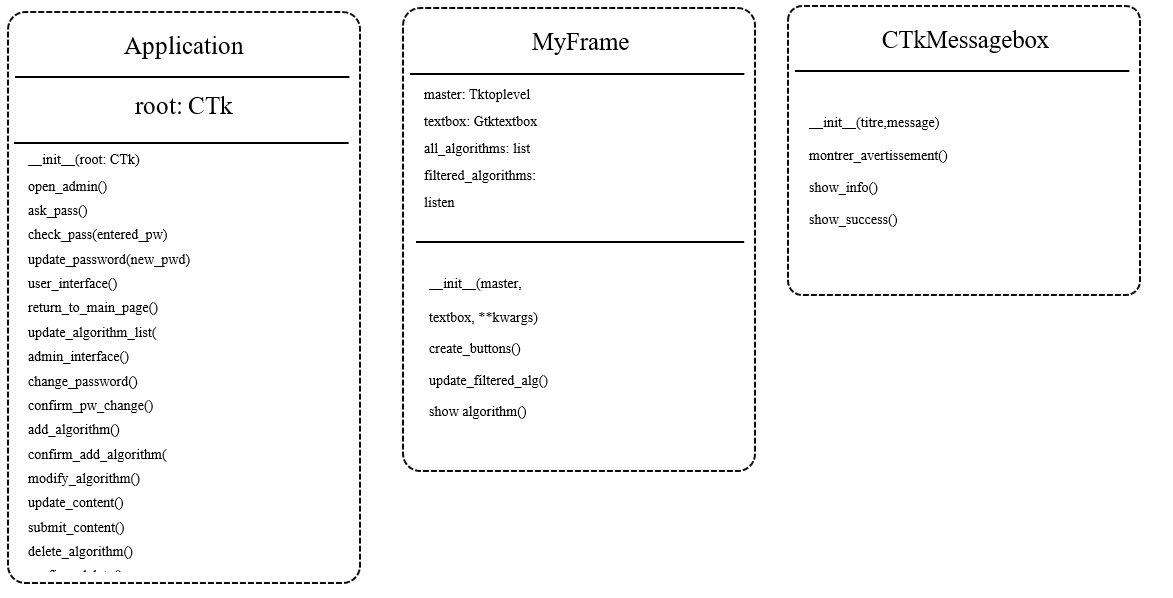
\includegraphics[width=0.9\linewidth]{images/classes}
	\caption{Диаграмма классов}
	\label{fig:classdiag}
\end{figure}


